\section{Introduction}

In the previous chapter, we saw the adoption of the carbon-aware technique follow-the-renewables applied to a multi-cloud distributed over a country, and the drawbacks it presents if not used properly, such as network congestion and extra energy consumption. Now, the reader is presented to another strategy: sizing (or dimensioning) the renewable infrastructure to reduce the carbon footprint of the cloud operation. This strategy consists of defining how much investment needs to be made, for example, defining the area of solar panels (when considering solar power), the number of wind turbines, and the capacity of the energy storage devices (such as lithium-ion batteries) that need to be manufactured. 

The scenario considered has some differences to better represent modern cloud providers. First, it is considered that the DCs are geographically distributed over the world, which represents real cloud providers such as Google, Microsoft, Facebook, and so on, as can be seen in Figure~\ref{fig:dc_locations}. Many reasons justifies the need for geographically distributed DCs: i) meet the demand for the ever-increasing number of users; ii) redundancy, for example if there is a problem in some region the workload can be shifted to another location; iii) reduce the latency or response time for the users. This geographic distribution also allows to better harvest the renewables sources, since there is a more variable climate conditions, solar irradiation levels is different between the countries, as well as the wind received. Second, many locations in the world have the presence of low carbon intensive sources in their local electricity grid, therefore in reality there is not only green and brown classification (as seen in the previous chapter). Classifying between brown and green made sense in the previous scenario since it was considered only a single country, and the renewable energy was less carbon intensive than the local electricity grid. Finally, energy storage devices can be used to store the overproduction of renewable energy and use it when opportune.

One point that cannot be neglected is that manufacturing the renewable infrastructure also presents a environmental impact: batteries have an ideal level of charge that can improve their lifetime, which can reduce the replacement frequency, but on the other hand, causes them to be oversized \cite{batteries_baumman}, and their recycles rates still need to improve \cite{bateries_RAHMAN}; and considering the current state-of-the-art PVs, if they produce 40\% of the global electricity by 2050, they will consume about 5\% of today’s ${CO_2}$ budget \cite{solar_co2}.

In this chapter, we explore the adoption of both strategies, sizing the PVs and batteries and scheduling with follow-the-renewables to reduce the carbon footprint of operating existing cloud platforms. More specifically, this chapter presents the following contributions: 

\begin{itemize}
    
    \item the two sub-problems---PVs and batteries sizing, and workload scheduling--- are modeled as a single problem, which allows evaluating scenarios such as: should the battery capacity or the PV area be increased, or should the workload be scheduled in a data center located in another part of the world?
    
    \item we propose a model that uses a linear programming approach (LP) with real variables, allowing us to optimally solve the problem we address in polynomial time using classical LP solvers. This allows a large number of scenarios to be evaluated over broad time horizons (i.e., one year) to take the seasonal behavior of renewable energy production into account. This model can be extended to multiple scenarios, and it may help decision-makers evaluate which regions need more investment to reduce the cloud operation's environmental impact.

\end{itemize}



The work of this chapter was done in collaboration with the following members of the DATAZERO\cite{datazero} research team: Georges da Costa, Jean-Marc Nicod and Veronika Rehn-Sonigo, and it resulted in the following publication:  \textit{\textbf{Vasconcelos, M.}, Cordeiro, D., Costa, G. D., Dufossé, F., Nicod, J.-M., and Rehn-Sonigo, V. (2023). Optimal sizing of a globally distributed low carbon cloud federation. In The 23rd IEEE/ACM International Symposium on Cluster, Cloud and Internet Computing}. The text of the present chapter is an adaptation of this publication.


The remainder of the chapter is organized as follows: Section~\ref{sec:problemStatement_ccgrid} defines the problem addressed, the assumptions, the models, and the objective function. Details about the problem constraints and how to optimally solve the problem are given in Section~\ref{sec:optimalresolution_ccgrid}. The experiments are presented in Section~\ref{sec:experiments_ccgrid} and their results are discussed in Section~\ref{sec:analysis-discussion_ccgrid}. Finally, Section~\ref{sec:conclusion_ccgrid} concludes the chapter. 



\section{Problem statement}
\label{sec:problemStatement_ccgrid}

This section describes the addressed problem and hypothesis. The next two sections further detail the modeling, notations, and the optimal approach to solve the decision problem that we tackle within the chapter. 

\subsection{Addressed problem}
\label{sec:addressedproblem_ccgrid}

As mentioned earlier, the goal is to reduce the carbon footprint of an existing cloud platform both in its operation and sizing the renewable infrastructure. The cloud platform consists of several data centers spread worldwide, in both hemispheres and on all continents. The proposed solution aims to design an additional solar-based power supply infrastructure to the classical power grid connection and to define an optimal way to operate the global IT cloud platform by scheduling its workload. To green the cloud infrastructure and reduce its carbon footprint, we must reduce the use of high-carbon-intensive energy to operate the data centers. Using renewable energy is a promising option, however, the carbon footprint of manufacturing needs to be taken into account.

Another problem is that the location where the DC is installed determines how sustainable it can be. First, the carbon intensity of the energy consumed from the local electricity grid depends on how it is produced: natural gas, coal combustion, hydraulic or nuclear energy. Second, each location has different climate conditions, and renewable power production will also have different efficiency. For example, solar power will be higher in locations that receive more solar irradiation, depending on whether it is near or far from the tropics. Therefore, powering the cloud federation is a balance or mix between using low-carbon electricity from the local grid and using its solar panels, with the understanding that batteries are mandatory to mitigate intrinsic solar power intermittency. 

The current decision problem aims to define the additional renewable power supply architecture from solar energy to reduce the carbon footprint of the global cloud infrastructure. It is assumed that: i) the data centers are already in operation, and the sizing will only define the area of PV panels and the capacity of the batteries; ii) the DCs can be supplied from the power of the local electricity grid, power from the PV panels or power stored in the batteries; iii) job submission is centralized; iv) 
100\% of the jobs must be completed in time (no delay); v) no migration of jobs; vi) jobs can be executed in any of the data centers; vii) cloud platform is homogeneous regarding the IT part (number of servers, CPU cores, and model, network equipment), but the total power consumption of the DCs is different because of the power used for cooling the DCs at each geographic location. Finally, the following inputs are considered:

\begin{itemize}
    \item specifications of the cloud infrastructure 
    \begin{itemize}
        \item number of servers, CPU cores per server, network switches
        \item power consumption of the servers (static and dynamic) and network equipment
        \item Power Usage Effectiveness (PUE) to represent cooling needs
    \end{itemize}
    
    \item specifications of the renewable infrastructure
    \begin{itemize}
        \item manufacturing carbon footprint
        \item technical parameters: batteries charge/discharge ratio and Max Depth of Discharge, PV efficiency to convert solar irradiation to power
    \end{itemize}
    \item weather conditions (solar irradiation) in areas where each data center operates for the federation (time series of 1 year with one value for every hour)
    \item carbon intensity of the local electricity grid in g CO2 eq per kWh for each DC
    \item the workload computing demand from clients (time series of 1 year with one value for every hour)

\end{itemize}

Now, the models and notations are introduced before the objective function to optimize.

\subsection{Models and notations}
\label{sec:modelsnotations_ccgrid}

\begin{table}[!t]
\caption{Main notations for the IT model for each $DC^d$ ($1\leq d\leq D$) during time slot $k$ ($0\leq k< K$)\label{table:variablesIT}}
\begin{center}
\begin{tabular}{l p{6cm}}

% Notations & Meaning\\

$\Delta t$ & time slot's time duration in the unit of time [$u.t$] \\
$\mathcal{H}$ & decision horizon $\mathcal{H} = K\Delta t$ \\
$K$ & number of time slots $\Delta t = 1\,\text{h} = 1\,u.t.$ \\ 
$k$ & time slot between dates $k\Delta t$ and $(k+1)\Delta t$ excluded \\ \\
$DC^d$ & a specific data center $d$ of the cloud federation \\
$\mathcal{DC}$ & the set of all data centers $\{DC^d \ | \ d=1, \ldots, D\}$ \\
$C^d$ & number of CPU cores within $DC^d$ \\
\\
$Pcore$ & dynamic power consumption of one CPU core at 100\% of utilization \\
$Pidle^d$ & static power consumption of all the servers of $DC^d$ \\
$Pintranet^d$ & power consumption of network devices of the $DC^d$  \\
$P_k^d$ & the power demand to perform tasks on $DC^d$ during time slot $k$ \\ 
$PUE^d$ & Power Usage Effectiveness of data center $d$\\ 
\\
$\mathcal{T}$ & the workload to execute ($ = \{ T_i\ |\ 1\leq i\leq N\}$) \\
$T_i$ & task $i$ of the workload $\mathcal{T}$ ($1\leq i\leq N$) \\
$r_i$ & release date of tasks $T_i$\\
$p_i$ & processing time of tasks $T_i$\\
$c_i$ & number of CPU cores needed to execute task $T_i$\\ 
$w_k$ & number of required CPU cores during the $k$th time slot \\
$w_k^d$ & number of CPU cores needed during the $k$th time slot on $DC^d$\\ \\\end{tabular}
\end{center}
\end{table}


To propose a solution for job operations, a decision horizon $\mathcal{H}$ is defined where job scheduling decisions can be taken. To do so, we propose discretizing $\mathcal{H}$ into $K$ indivisible time slots with a duration of $\Delta t$ such that $\mathcal{H} = K\times\Delta t$. To simplify the notations, we consider $\Delta t = 1 u.t.$ (unit of time). In our experiments, we will assume that $\Delta t = 1h$ such that $K = 8760\,h$ with $\mathcal{H} = 1$ year. 
Let $k$ be the time slot index that addresses any instant $t$ such that $k\Delta t\leq t < (k+1)\Delta t$ with $0\leq k< K$. 


\subsubsection{IT part model} 

Let $\mathcal{DC} = \{DC^d \ | \ d=1, \ldots, D\}$ be the set of data centers in the cloud federation. Considering a given data center $DC^d$, let $C^d$ be its number of CPU cores and $Pcore$ the energy used to power one core.


The power consumption of a cloud data center can be classified as static or dynamic~\cite{ahvar22_estimating_cloud_cons}. For the static part, the current model considers the idle power consumption $Pidle^d$ of the servers, the Power Usage Effectiveness (PUE) to represent the power consumption used to cool the DC infrastructure, and the power consumption of the network switches $Pintranet^d$ that interconnect the servers in each data center $DC^d$. Regarding the latter, cloud data centers usually adopt the fat-tree topology to interconnect servers in the DC~\cite{ahvar22_estimating_cloud_cons}. In this topology, one can compute the number of network switches needed to match the number of servers. The power consumption of the network switches is considered to be static based on actual measurements, which have shown that the consumption does not change significantly with the device usage~\cite{Hlavacs2009_energy_network_devices}. Moreover, each geographic location has different cooling needs, therefore each DC has a specific $PUE^d$ value. 

Finally, the dynamic part of the power consumption is represented by the additional power demand generated by using the CPU cores in each data center --- to execute the workload $ w^d_k$ assigned to the DC $d$ at time slot $k$ . Equation~\eqref{eq:power_cons} represents the power consumption of each DC for each step $k$ ($0\leq k<K$):

\begin{equation} \label{eq:power_cons}
   P^d_k  = PUE^d \times \big( Pidle^d + Pintranet^d + Pcore \times w^d_k\big)
\end{equation}



\subsubsection{Workload model}

Considering the workload that needs to be executed, let $\mathcal{T} = \{T_i \ | \ i=1, \ldots, N\}$ be the set of $N$ tasks that have to finish in time during the time horizon $\mathcal{H}$. Each task $T_i$ has the following properties: i) release date $r_i$; ii)  processing time $p_i$;  and iii) needs $c_i$ CPU cores at 100\% of usage to be executed. Let $w_k$ be the total number of CPU cores needed to compute tasks during the time slot $k$ in order to complete the workload in time. At each time step, $w_k$ is the sum over all cores required by the tasks executed in time slot $k$, and given that the tasks will be scheduled to the DCs,  $w_k^d$ is the sum of the number of cores used to execute the allocated workload in $\mathcal{DC}$ (with $1\leq d\leq D)$ and $0\leq k<K$) as shown by Equation~\eqref{eq:wk}:

\begin{equation} \label{eq:wk}
    w_k = \sum_{T_i|r_i\leq k\Delta t<r_i+p_i} c_i = \sum_d w_k^d
\end{equation}


\subsubsection{Electrical part model}

\begin{table}[t]
\caption{Main notations for the Electrical part model of each $DC^d$ ($1\leq d\leq D$) during each time step $k$ ($0\leq k<K$)\label{table:variablesElec}}
\begin{center}
\begin{tabular}{l p{6cm}}
%Notations & Meaning\\
$I^d_k$ & solar irradiation at time slot $k$ [$Wh/m^2$] \\
$Apv^d$ & surface area of photovoltaic panels of DC $DC^d$ [$m^2$] \\ 
$\eta_{pv}$ & PV efficiency (in \%) in converting solar irradiation to power \\
\\
$Pgrid_k^d$ & power consumed from the grid at time slot $k$ [$W$]\\
$Pre_k^d$ & power generated from the PVs at time slot $k$ [$W$] \\
\\
$BAT^d$ & battery capacity installed in $DC^d$ [$Wh$] \\
$B_k^k$ & battery level of energy at the time $k\times\Delta t$ [$Wh$] \\
$Pch_k^d$ & power charged in the batteries during time slot $k$ [$W$]\\
$Pdch_k^d$ & power discharged from the batteries during time slot $k$ [$W$] \\
$\eta_{ch}$ & efficiency of the charging process  \\
$\eta_{dch}$ & efficiency of the discharging process  \\

\end{tabular}
\end{center}
\end{table}

The power supply of the whole cloud platform $\mathcal{DC}$ has three sources: i) the renewable energy generated by the solar panels (PVs) installed on each $DC^d$ site; ii)  the classical electrical grid $Pgrid_k^d$ of each country on which $DC^d\in\mathcal{D}$ is hosted --- used as backup when the power from the renewable infrastructure is not enough; and iii) energy discharged from the energy storage devices. The storage devices are mandatory to mitigate the intermittency of solar power by storing the overproduction when the sun shines to provide energy during the night when the solar panels do not produce power. Lithium-Ion batteries have been chosen to play this role because of their good efficiency in terms of costs, power and energy density, charge and discharge rates, and self-discharge~\cite{wang2012_EDCS}. To model the fact that the cloud platform will not sell back energy to the grid, there is the constraint that the power from the grid ($Pgrid^d_k$) is always positive. 

Equation~\eqref{eq:predk} models the on-site renewable power production,  it depends on the solar irradiation $I^d_k$ received at the location of $DC^d$ during the time slot $k$, on the surface area of the solar panels $Apv^d$ and on the efficiency $\eta_{pv}$ of the PVs. 

\begin{equation} \label{eq:predk}
    Pre^d_{k}= I^d_k \times Apv^d \times \eta_{pv}
\end{equation}


Batteries are systematically installed next to the PVs for the reason mentioned above. Let $B^d_k$ be the battery level of energy, that is, the amount of energy (in $Wh$) at time $k\time\Delta t$ stored in batteries of capacity $BAT^d$ installed in $DC^d$ ($B^d_0 = Binit^d$ being the amount of energy at the beginning the time horizon $\mathcal{H}$). The variable $Pch_k^d$ represents the power charged in the batteries of DC $d$ during the time slot $k$ (and $Pdch_k^d$ is the power discharged from the batteries). It is not possible to charge and discharge simultaneously: if $Pch^d_k$ is greater than zero, $Pdch^d_k$ equals zero and vice versa. Regarding the batteries modeling, the charging and discharging process has an efficiency $\eta_{ch}$ and $\eta_{dch}$ less than 1. Lithium-Ion batteries have a low value for daily self-discharge (0.5\,\% per day)~\cite{wang2012_EDCS}, thus this property was not modeled. Finally, to increase the lifetime, the batteries cannot be discharged more than its Maximum Depth of Discharge. 

Equation~\eqref{eq:bdk} models the battery in terms of the level of energy:

\begin{equation} \label{eq:bdk}
  B^d_k = B^d_{k-1}  + Pch^d_{k-1} \times \eta_{ch} \times \Delta{t} - \frac{Pdch^d_{k-1}}{\eta_{dch}} \times \Delta{t}
\end{equation}
with $0.2\times BAT^d \leq B^d_k\leq 0.8\times BAT^d$ for any time slot $k$ and $DC^d$ ($0\leq k<K$ and $1\leq d\leq D$) --- this last restriction models the Max Depth of Discharge property to increase the battery lifespan. The modeling of the batteries and PVs are based on~\cite{2021NICOD_ILP}.


\subsubsection{Footprint model} \label{sec:footprintmodel_ccgrid}


In the current model, carbon emissions from operating the cloud platform originate from three sources: (i) consuming power from the regular electrical grid and manufacturing of both (ii) the photovoltaic panels, and (iii) the batteries. Equation~\eqref{eq:fpgrid} models the carbon footprint of the regular local electrical grid, defined by the carbon intensity of the power grid $gridCO2^d$ in the region of data center $DC^d$  times the amount of energy used during the time slot $k$.

\begin{equation} \label{eq:fpgrid}
FPgrid_k^d = Pgrid_k^d\times \Delta t \times gridCO2^d
\end{equation}

It is considered that the power from the local electricity grid may originate from multiple sources, and the $gridCO2^d$ is an input that represents its average carbon intensity during the year: the value will be low if it is supplied by solar, wind power, hydroelectric or nuclear power. On the other hand, the value will be higher if it is supplied by coal, oil, biomass, or natural gas.

For the carbon footprint of the PVs, to account for the different climate conditions at each region, in particular the solar irradiation received, one must also consider the expected power output that PVs can produce over their lifetime, as using a single year may cause over or under-sizing of the PV infrastructure. Therefore, the carbon footprint of PVs is also related to the location of each data center. Equation~\eqref{eq:pvco2} models the carbon footprint for PVs:

\begin{equation} \label{eq:pvco2}
   pvCO2^d =  \frac{FPpv_{1m2}}{expectedEpv^d} 
\end{equation}

where $FPpv_{1m2}$ is the emissions of manufacturing $1\,m^2$ PV in $g\,\ch{CO2}-eq$, and $expectedEpv^d$ is the expected energy production in $Wh$ that $1\,m^2$ of the PV during its lifetime at the location of $DC^d$. As a result, the unit of this metric is expressed in $g\,\ch{CO2}-eq.Wh^{-1}$, and so, the total emissions from the PVs are related to its power production, as shown in Equation~\eqref{eq:fppvdk}. 

\begin{equation} \label{eq:fppvdk}
   FPpv^d_k =  pvCO2^d \times Pre_k^d \times \Delta t
\end{equation}


Regarding the batteries' carbon footprint $FPbat^d$ of the DC $DC^d$, it is computed based in their capacity $BAT^d$ ($kWh$) and the carbon emissions of the manufacturing process $batCOS$ in $g\,\ch{CO2}-eq.kWh^{-1}$, as seen in Equation~\eqref{eq:fbat}. To be consistent with the calculation of $FPpv^d_k$, $batCO2$ is the share of the carbon footprint of the battery type chosen for a capacity of $1\,kWh$ over the time horizon of $\mathcal{H}$, assuming a battery has a lifetime of 10 years. Thus, given that we are considering one year of cloud operation, $batCO2$ is the tenth of the total carbon footprint of the considered battery. It is considered that the battery carbon footprint is homogeneous for all the locations, as the climate conditions do not influence it.


\begin{equation} \label{eq:fbat}
   FPbat^d =  BAT^d \times batCO2
\end{equation}


These modifications regarding the lifetime of PVs and batteries were necessary because we are considering only one year of cloud operation. Suppose we use the total carbon emissions for manufacturing the PVs and batteries. In that case, the solver will find a solution where there is little to no PV or batteries, because using the regular electrical grid would be less carbon-intensive.  

\subsection{Objective function}
\label{sec:objectivefunction_ccgrid}

Now that the reader has been introduced to the modeling of the problem, the objective function can be defined (see Equation~\eqref{eq:FPALL}). It consists of minimizing the carbon footprint of the globally distributed cloud federation to reduce as much as possible the carbon emissions, which come from both the consumption of electricity from the power grid, as well as from the manufacturing of photovoltaic panels and batteries with $k$ and $d$ defined as follows: $0\leq k< K$ and $1\leq d\leq D$.

\begin{equation} \label{eq:FPALL}
\text{minimize }\sum_{k=0}^{K-1} \sum_{d=1}^D ( FPgrid^d_k +  FPpv^d_k) + \sum_{d=1}^D FPbat^d
\end{equation}


\section{Optimal resolution}
\label{sec:optimalresolution_ccgrid}


In this section, we show that linear expressions can be used to express the constraints governing the operation of the globally distributed cloud platform. This is a mandatory step, since all the models presented in the previous section are linear equations. New real variables and constraints are introduced to finish building the linear program that needs to be solved to achieve the targeted objective (see Equation~\eqref{eq:FPALL}). The solution obtained after solving the linear program is optimal in nature and computed in polynomial time, as the model uses only real variables. Polynomial time is mandatory if we consider the number of variables needed for a time horizon $\mathcal{H}$ as long as one year (with time slots of 1 hour). We assume to choose real positive values for all variables even if variables denote discrete objects like cores. Indeed, $w_k^d$ is the number of cores needed to run tasks on $DC^d$ during time slot $k$. Considering the size of modern cloud data centers with thousands of servers and millions of cores, the decimal part of each $w_k^d$ can be neglected. Having the solution with more or less than a core on a given DC keeps the order of magnitude for the PV and battery sizing process the same. Finally, some constraints are explicit, and others are implicit to avoid the addition of integer variables, which would transform this LP into a MILP whose solving process would not scale at all.


\subsection{Constraints to address the workload}

The workload to be executed must respect each data center's computational capabilities $C^d$ (number of available CPU cores). Equation~\eqref{eq:wkcd} expresses that the number of cores that will be allocated to execute the tasks of the workload ($w_k^d$) does not exceed the existing number of cores of $DC^d$:

\begin{equation}\label{eq:wkcd}
    w_k^d \leq C^d
\end{equation}


\subsection{Constraints to reach the power demand}

The electric part of each DC has to supply the DC power demand using local renewable energy from its PV panels ($Pre_k^d$), from batteries ($Pdch_k^d$ and $Pch_k^d$) and/or from the classical electrical grid ($Pgrid_k^d$). Equation~\eqref{eq:pkdconstraint} presents the restriction for the power consumption.

\begin{equation} \label{eq:pkdconstraint}
    P^d_k \leq Pre^d_k + Pgrid^d_k + Pdch_k^d - Pch_k^d
\end{equation}

\subsection{Constraints on batteries}

The batteries are defined by their capacity ( $BAT^d$ in kWh), and each data center can have a different size of batteries depending on how the intermittency of the renewable energies is managed on each site, for example, if the local electricity grid is high-carbon intensive, the battery will need a higher capacity in order to store solar power during the day to use it during night, otherwise if the local electricity grid has the presence of low-carbon intensive sources, the battery will have a smaller capacity. Equation~\eqref{eq:batlimit} models the Max Depth of Discharge property, that is, the range that the battery needs to operate in order to increase its lifetime. In addition, the power to charge or discharge a battery is also limited by the level of energy remaining in the associated battery, so it is not possible to reach a forbidden energy level. Equations~\eqref{eq:pchlimit} and~\eqref{eq:pdchlimit} express these constraints.

\begin{equation} \label{eq:batlimit}
0.2\times BAT^d\leq B_k^d\leq 0.8\times BAT^d
\end{equation}
\begin{equation} \label{eq:pchlimit}
Pch^d_k \times \Delta t \times \eta_{ch} \leq 0.8\times BAT^d - B^d_{k-1}
\end{equation}
\begin{equation} \label{eq:pdchlimit}
Pdch^d_k \times \Delta t\ / \ \eta_{dch} \leq B^d_{k-1} - 0.2\times BAT^d
\end{equation}


The reader may notice the absence of restrictions for charging and discharging simultaneously in the modeling. Such restrictions would impose the usage of binary variables that would significantly increase the required computational time to find the optimal solution to the problem. We performed experiments with a shorter duration (around one month), and the sizing results were the same between both versions: using and not using binary variables. Furthermore, given a solution for the linear program, it is possible to calculate an alternative solution program where there would be no charge and discharge at the same time slot and with the same sizing results --- the differences between the solutions would be the values of the variables $Pch_k^d$ and $Pdch_k^d$.


\subsection{Linear program}

The following linear program (LP) summarises what has been described in the current section concerning the model to solve the tackled problem. After solving the LP, the values of the variables are used to define both the renewable power supply part completely --- variables $BAT^d$ for the battery capacity and $Apv^d$ for the area of the solar panels at each $DC^d$  --- and the core operating process of the distributed low carbon cloud federation with details of the way each DC is used time slot by time slot for one year on the considered weather conditions --- variables $ w_k^d$ that represents the workload scheduled and $Pch^d_k$ (and $Pdch^d_k$) for the power charged into (and discharged from) the batteries of each $DC^d$ at each time slot $k$. Comprehensive experiments have been led to highlight the pertinence of the approach. These experiments are shown in the next section, and a discussion is proposed in Section~\ref{sec:analysis-discussion_ccgrid}.

\begin{equation}\nonumber
    \text{(LP)}\left\{
    \begin{array}{ll}
        \text{minimize}\displaystyle\sum_{k=0}^{K-1}\sum_{d=1}^D (FPgrid^d_k\!+\!FPpv^d_k)\!+\!\sum_{d=1}^D FPbat^d \label{eq:lp}\\ \\
        \text{s.t. } \ \ \ \ 
\eqref{eq:power_cons}\,\eqref{eq:predk}\,\eqref{eq:bdk}\,\eqref{eq:fpgrid}\,\eqref{eq:fppvdk}\,\eqref{eq:fbat}\,\eqref{eq:wkcd}\,\eqref{eq:pkdconstraint}\,\eqref{eq:batlimit}\,\eqref{eq:pchlimit}\,\eqref{eq:pdchlimit} %\nonumber
    \end{array}
    \right.
\end{equation}

where all variables are positive real variables. 


\section{Experiments}
\label{sec:experiments_ccgrid}

In this section, we present the settings and the results of the
experiments.  More details for reproducing the experiments can be
found in the public available software artifact \cite{artifact_ccgrid}. 

\subsection{Settings}


\label{sec:settings_ccgrid}


\subsubsection{Cloud infrastructure}

The servers are homogeneous and based on equipment of real cloud infrastructure: the Taurus server of the Grid'5000 testbed\footnote{\url{https://www.grid5000.fr/w/Lyon:Hardware\#taurus}}. The servers are equipped with two Intel Xeon E2630 CPUs, with a total of 12 CPU cores. For modeling the power consumption of the servers, real measurements conducted by~\cite{ahvar22_estimating_cloud_cons} were considered: in the idle state, each server consumes 97\,W, and their maximum power consumption (when using 100\% of the 12 cores) is 220\,W. The value of Pcore is 10.25\,W, and it was obtained by linear interpolation between the power consumption of the idle and the fully used state.

Each data center is equipped with 23,200 servers (and a total of 278,400 cores). This number represents what can be seen in production data centers of major cloud players: Microsoft operates over 4 million servers distributed over 200 DCs~\cite{roach2021_microsoftazure}. The total power consumption from the servers of each data center when idle is 2.25\,MW, and their maximum power consumption is 5.1\,MW.

For the current experiments, we considered a network with a 48-ary fat-tree topology for the interconnection of the servers inside the DCs, that is, the network switches have 48 ports, and the total number of switches is 2,880. The power consumption of the switches was based on real measurements by~\citet{Hlavacs2009_energy_network_devices}: the HP ProCurve 2810-48G was selected, with 48 ports and approximately 52W per device. In total, the network equipment power consumption is 149.76\,kW for each DC.

The locations of the data centers were based on the real cloud infrastructure of Microsoft Azure\footnote{Azure global infrastructure: \url{https://infrastructuremap.microsoft.com/}.}, and different regions in different continents, hemispheres, and time zones were selected. Figure~\ref{fig:dc_location} presents the details of the locations.


\begin{figure}[!htbp]
%\vspace{22pt}

\begin{picture}(300,300)

\put(0,0){
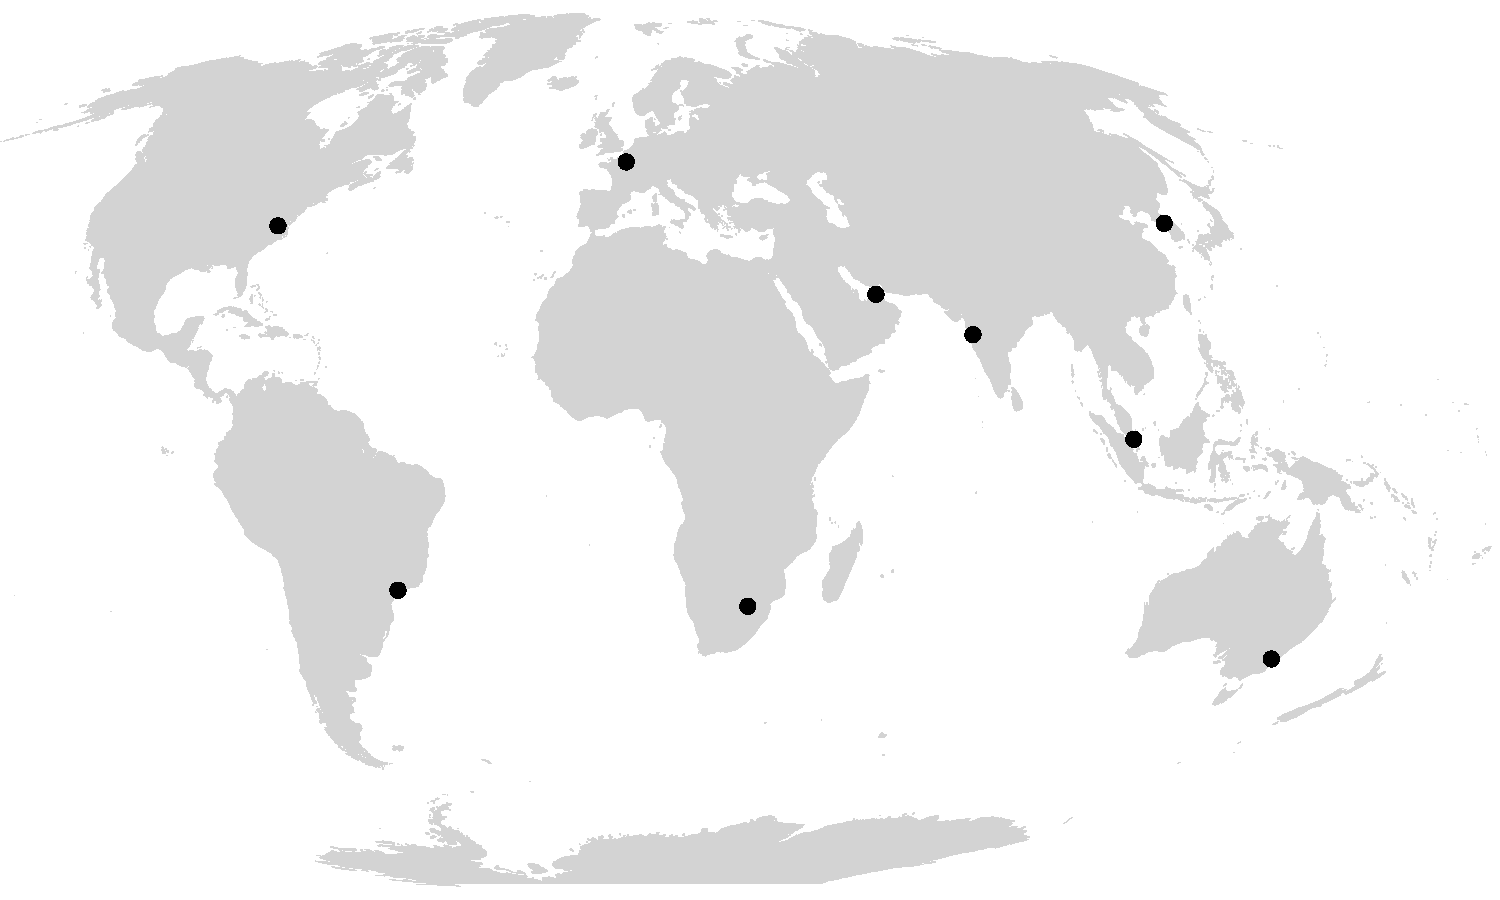
\includegraphics[width=\textwidth]{images/locations.pdf}

}

\put(45,160){Virginia, USA}
\put(60,70){São Paulo, BR}
\put(120,185){Paris, FR}
\put(180,60){Johannesburg, ZA}
\put(180,145){Dubai, UAE}
\put(255,135){Pune, IN}
\put(300,165){Seoul, KR}
\put(290,105){Singapore, SG}
\put(330,50){Canberra, AU}

\end{picture}

\caption{Selected locations for the data centers.}
\label{fig:dc_location}
\end{figure}


In order to represent the fact that each geographic region has different cooling needs, we used values for the PUE inspired by real data from Microsoft Azure for each site: for the Americas, the PUE is 1.17 (DCs São Paulo and Virginia), Asia Pacific has a PUE of 1.405 (DCs Pune, Canberra, Singapore, and Seoul), and for the Europe region, Middle East, Africa the PUE is 1.185 (DCs Johannesburg, Dubai, and Paris)~\cite{walsh2022_azurepue}. 

\subsubsection{Workload}

The workload used was created using the Grog generator\footnote{\url{https://pypi.org/project/grog/}},  a workload generator tool based on analysis of properties of the execution trace made available by Google in 2011~\cite{DACOSTA2018_grog}. For reproducibility purposes, the parameters regarding the number of tasks were set to 350,000, and the duration was 30 days. The workload generator was run 12 times --- 1 per month. Finally, the tasks have a duration of one hour.

\subsubsection{Photovoltaic power production}

The data for simulating the solar power production --- Global Solar Horizontal Irradiation (in Wh/m$^{2}$) --- was collected from the MERRA-2 project~\cite{GELARO2017MERRA2}, since it provides information for anywhere on earth. Figure~\ref{fig:pv_ghi} illustrates the average solar irradiation of each location throughout the year 2021.

 \begin{figure}[!htbp]
  \centering
   {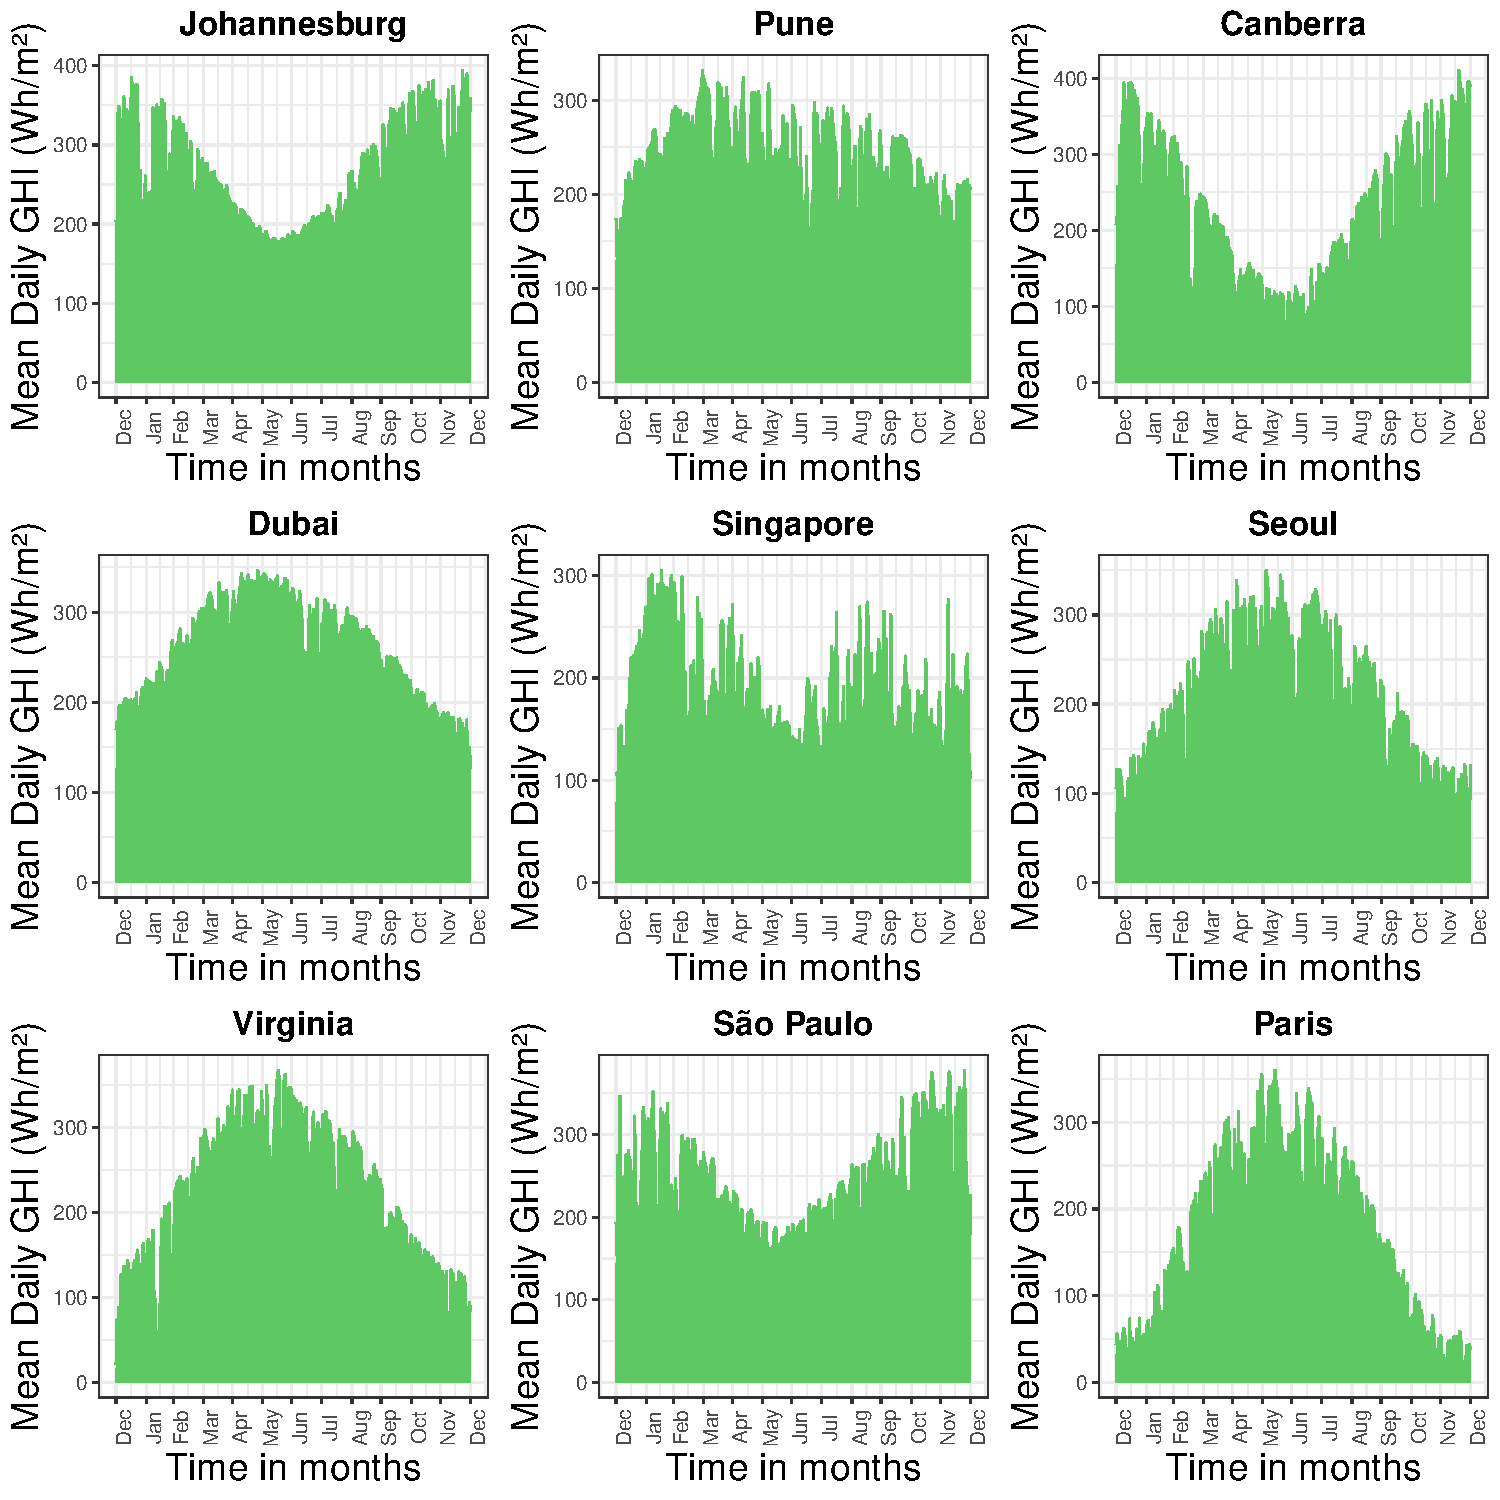
\epsfig{file = images/pv_ghi.pdf, width = \linewidth}}
  \caption{Average daily solar irradiation per location throughout the year 2021.}
  \label{fig:pv_ghi}
\end{figure}

\subsubsection{Carbon footprint}

For PV panels, it is considered a lifetime of 30 years, and manufacturing 1 $m^2$ emits $250 kg\,\ch{CO2}-eq$, inspired from real measurements~\cite{YUE2014pv_carbon}. To compute the emissions in the form of $g\,\ch{CO2}-eq.kWh^{-1}$ as stated in Section~\ref{sec:footprintmodel_ccgrid}, we considered the total solar irradiation that was produced during the year 2021 multiplied by 30 (to account for the PV module lifetime of 30 years). For the electrical grid, we also considered the real-world data of the carbon footprint ($g\,\ch{CO2}-eq.kWh^{-1}$). Table~\ref{tab:carbonfootprint} lists the carbon emission values for each region.
 %TODO Add text saying that the pv emissions considers the grid....

\begin{table}

  \caption{Emissions (in $g\,\ch{CO2}-eq.kWh^{-1}$) for both PV usage and using the regular grid. Source for grid emissions: electricityMap, climate-transparency.org.}\label{tab:carbonfootprint} \centering
  \begin{tabular}{|l|r|r|}
    
  \hline
    
  \textbf{Location} &  \textbf{Grid} & \textbf{PV} \\
  \hline
  Johannesburg & 900.6 & 24.90 \\
  \hline
  Pune & 702.8 & 27.96 \\
  \hline
  Canberra & 667.0 & 29.71 \\
  \hline
  Dubai & 530.0  & 24.84 \\
  \hline
  Singapore & 495.0 & 36.19 \\
  \hline     
  Seoul & 415.6 & 34.00 \\
  \hline
  Virginia  & 342.8 & 31.71 \\
  \hline
  São Paulo &  61.7 & 27.99\\
  \hline 
  Paris &  52.6  & 39.93 \\
  \hline  

\end{tabular}  
\end{table}

Regarding the batteries, the emissions are only considered for the manufacturing step---$59 kg\,\ch{CO2}-eq$ per kWh and are the same for all the DCs locations. In our experiments, the considered lifetime of the batteries is ten years. Therefore, the input used is equal to $5.9 kg\,\ch{CO2}-eq$ per kWh, given that we simulated one year.

\subsubsection{Execution environment}
 
The experiments were executed on a machine with the following configurations: Intel i9-11950H CPU, and 32 GB of RAM. The solver program used for solving the LP was the Gurobi Optimizer (version 9.5.2). The execution time for solving the LP with the inputs listed in the previous sections---which resulted in a total of 394,263 variables---was in the order of 30 seconds.

\subsection{Results}

In this section, we present the results in terms of the computed optimal area of the PVs and capacity of the batteries, the origin of energy used to supply the DCs operation (from the electrical grid, batteries, or PV panels), and the total emissions of the cloud operation, generated from both manufacturing PVs and batteries, and power consumption of the regular electrical grid. Furthermore, to assess the solution computed by the LP, we compare it with two other scenarios: i) DCs can only be supplied using power from the regular electrical grid --- representing most of the DCs in operation, and ii) only power generated from the PV panels, and stored and discharged from the batteries are used to supply the DCs --- represent green DCs that fully autonomous from the power grid. Finally, we present an evaluation using metrics to assess the environmental impact of the results.


\begin{figure}[!htbp]
  \centering
  {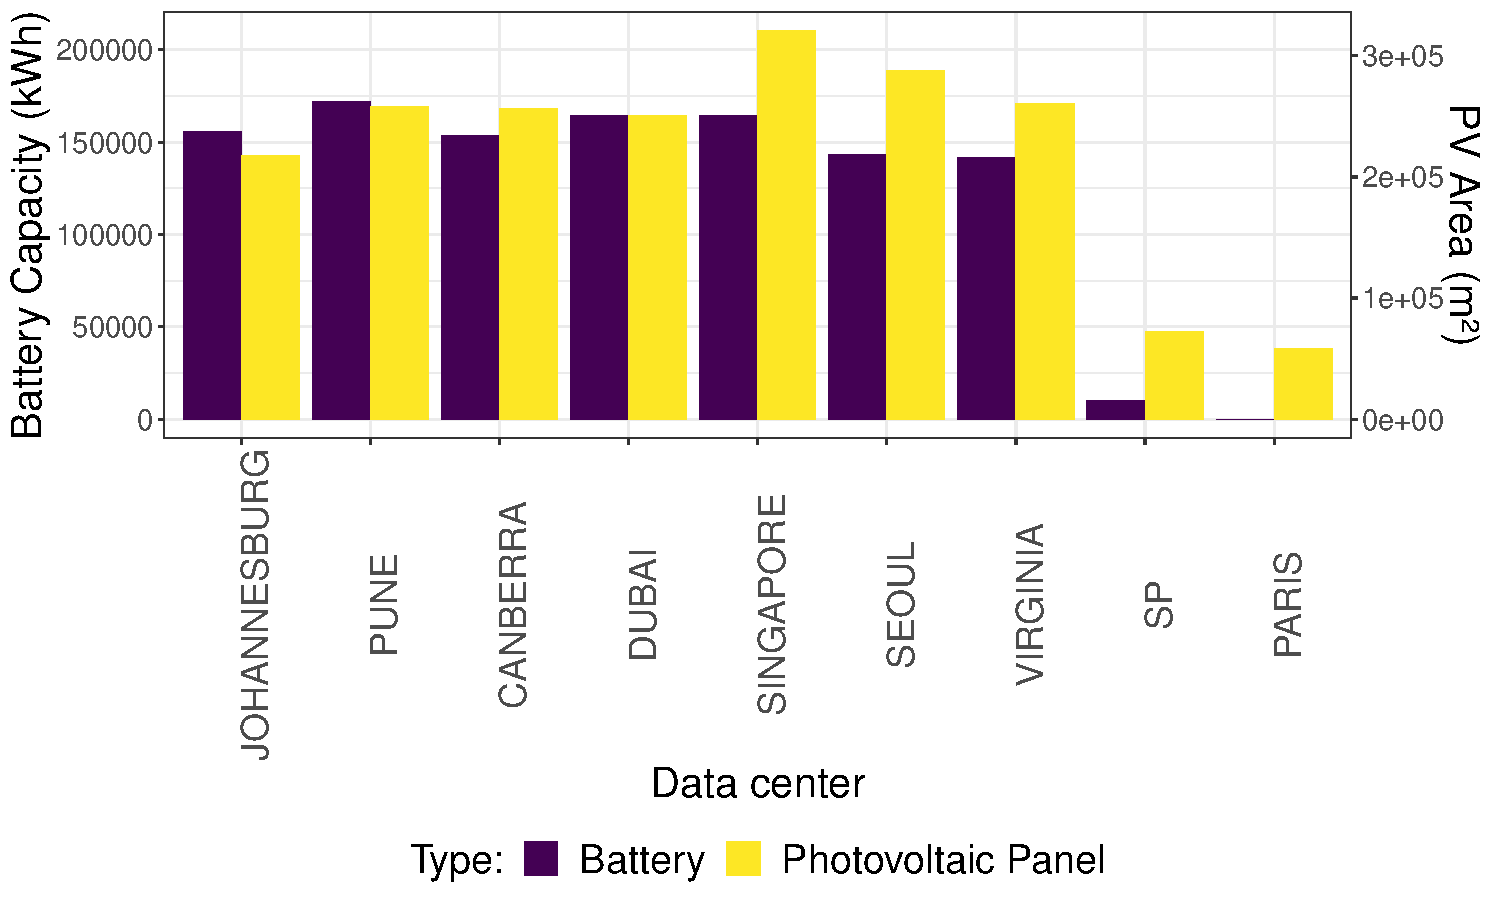
\epsfig{file = images/sizing.pdf, width = \textwidth}}
  \caption{Optimal result for the area of PV panels and capacity of the batteries.}
  \label{fig:sizing}
\end{figure}

Figure~\ref{fig:sizing} illustrates the optimal area of the photovoltaic panels and the capacity of the batteries computed from the LP using the inputs described in Section~\ref{sec:experiments_ccgrid}.

To analyze the sources of energy that supplied the DCs operation, we present in Figure~\ref{fig:energy_ratio_daily} the percentage that each source (grid, renewable, and batteries) was used to daily supply the DCs throughout the year. Figure~\ref{fig:power_ratio_hourly} is a fine-grain visualization of the DC operation regarding the power consumed or produced for one day (January 1st, 2021): it illustrates hour-by-hour the DC total power demand, how much power was consumed from the grid, discharged from the batteries, and produced by the PV panels.
 

\begin{figure}[!htbp]
  \centering
   {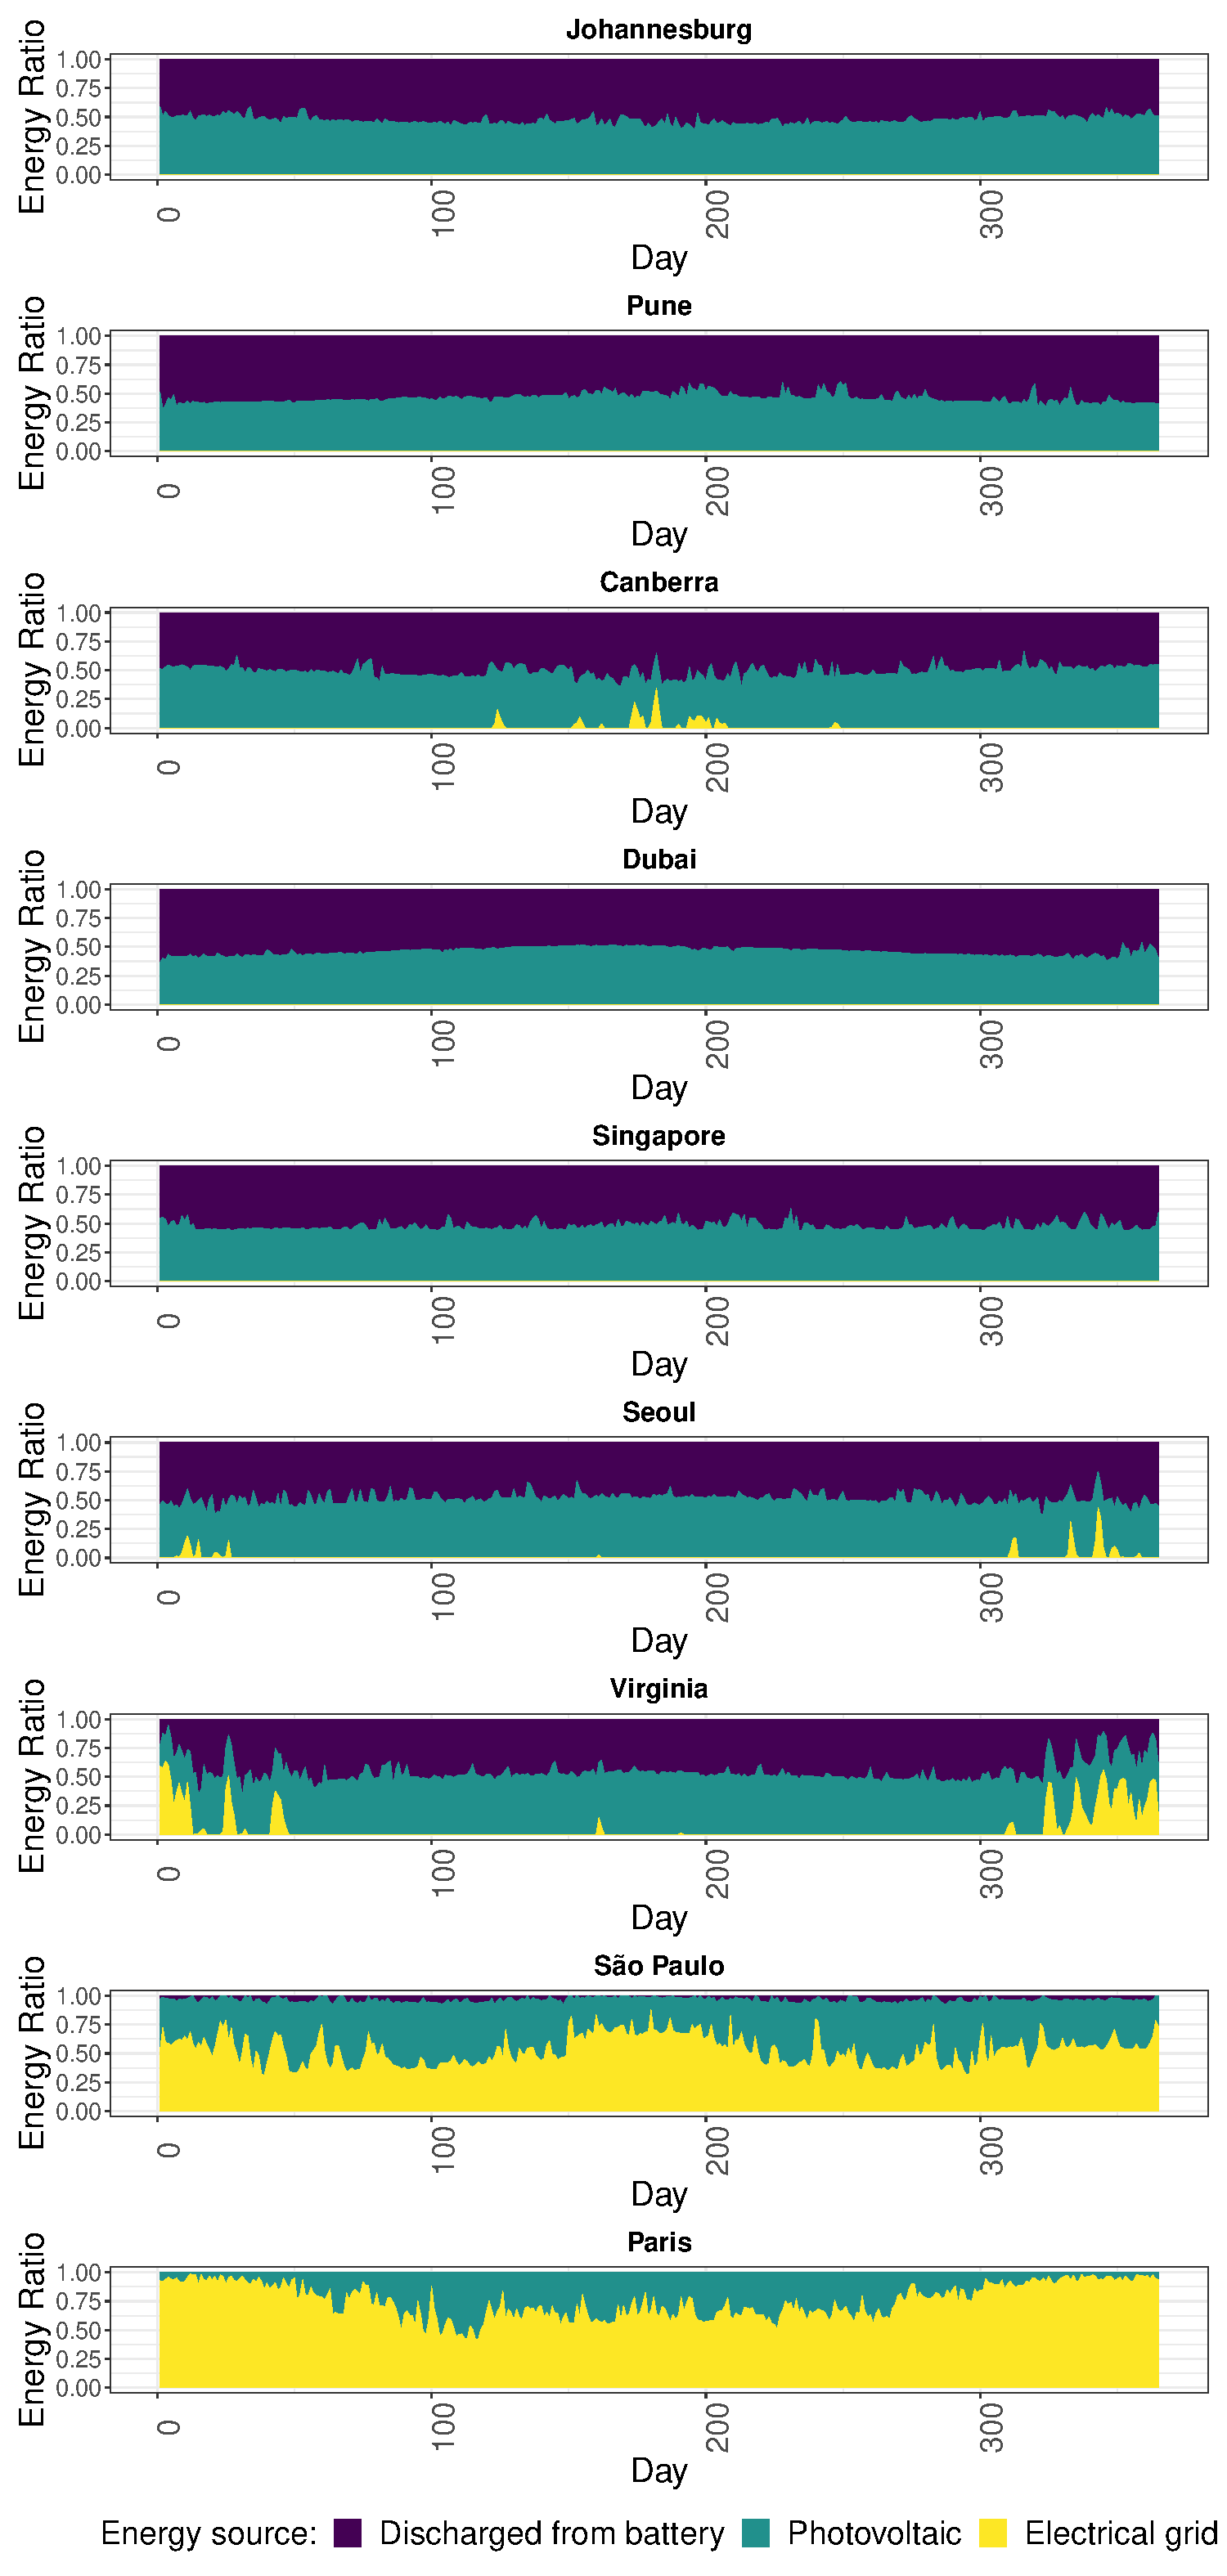
\epsfig{file = images/energy_ratio.pdf, width = .8\textwidth}}
  \caption{Composition of the DCs' daily energy consumption throughout the year considering the different sources of energy, where 1.0 is the DC's total energy consumption.}
  \label{fig:energy_ratio_daily}
\end{figure}




 \begin{figure}[!htbp]
  \centering
   {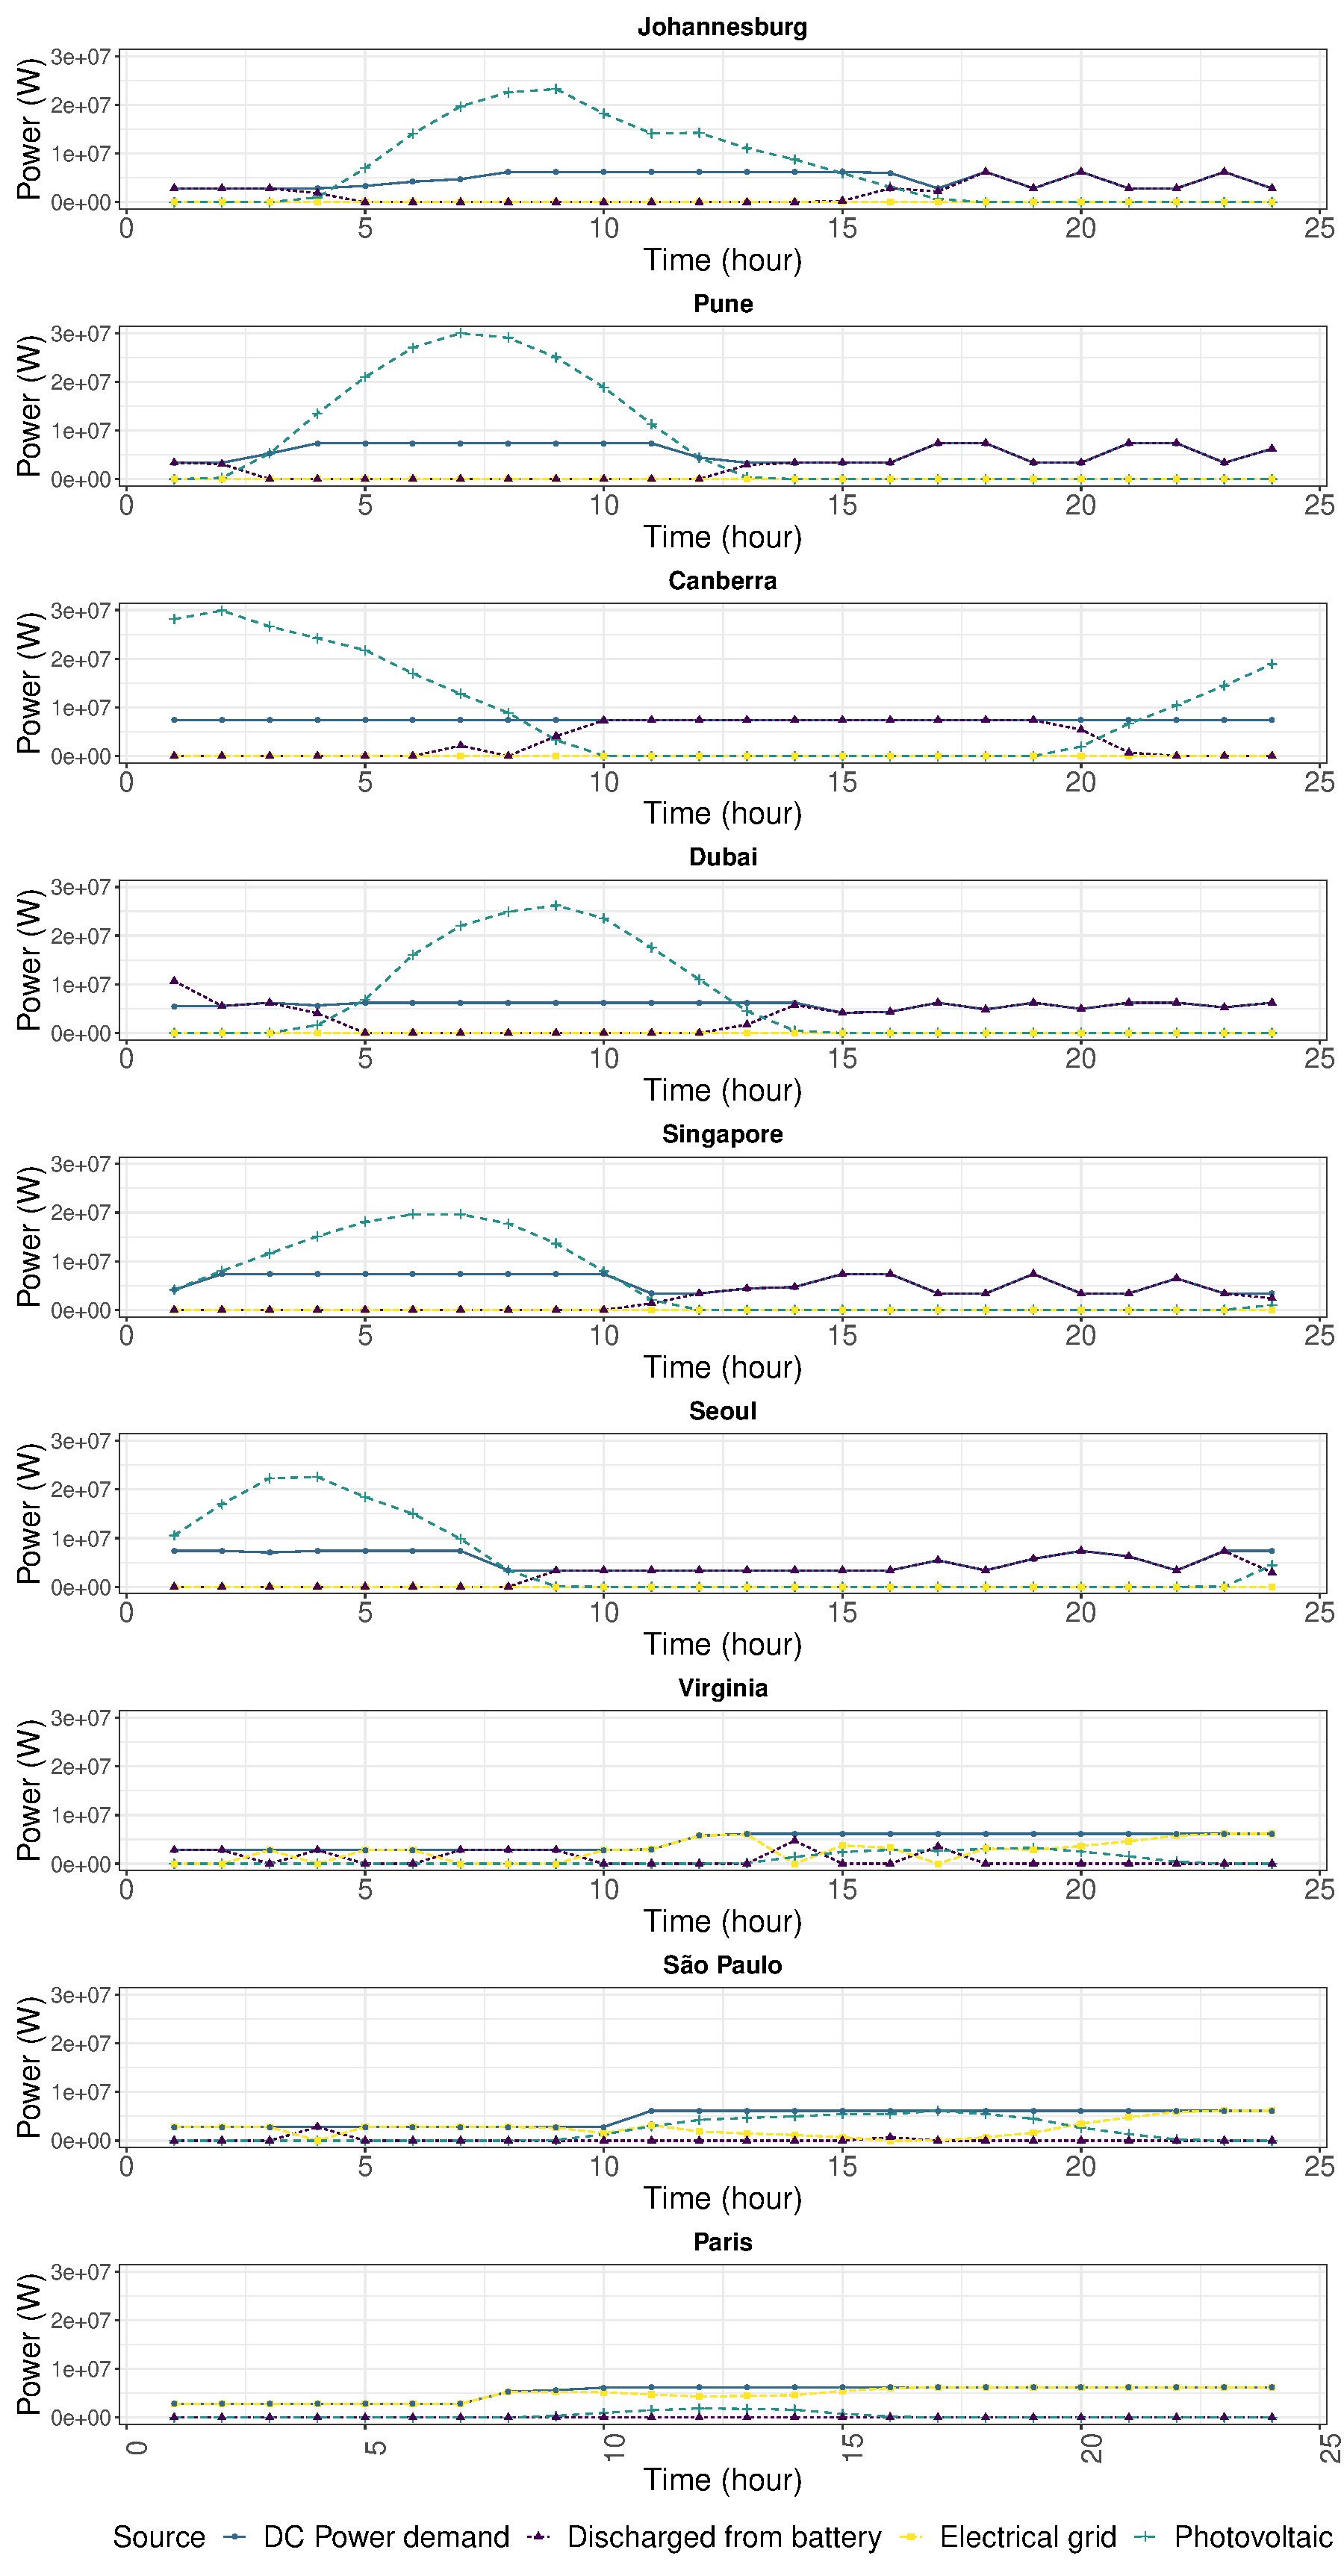
\epsfig{file = images/power_source_hour.pdf, width = .85\textwidth}}
  \caption{Composition of the DCs' hourly power consumption throughout the first day of the year. Time follows the Universal Time (UT) standard.}
  \label{fig:power_ratio_hourly}
\end{figure}

In order to assess the optimal solution of the LP, we compared it with two other scenarios in terms of total carbon emissions ($t\,\ch{CO2}-eq$): i) the DCs are only supplied by power from the regular electrical grid, and ii) the DCs are only supplied by renewable power from the photovoltaic panels and batteries. Table~\ref{tab:emissions} presents the results. In comparison with the first scenario (only grid power), the reduction in the \ch{CO2} emissions was approximately 85\%, and it was approximately 30\% for the second scenario (only renewable power).


\begin{table}[!ht]
\caption{Total emissions for the different scenarios.}\label{tab:emissions} \centering
\begin{tabular}{|p{5cm}|r|}
  \hline
  \textbf{Scenarios} & \textbf{Emissions ($t\,\ch{CO2}-eq$)}   \\
  \hline
  Electrical grid                    & 201 211.3    \\
  \hline
  PV and batteries  &                  42 370.6 \\ 
  \hline
  PV, batteries, and grid            &  29 600.6   \\
  \hline


\end{tabular}
\end{table}

To further evaluate these scenarios, we present in Table~\ref{tab:dcutilization} results in terms of the average load each DC executed throughout the year. Equation~\eqref{eq:dcload} represents how the metric was computed for each DC $d$. One may notice that the Johannesburg DC received no load for the scenario where only grid power is used. This is justified by two reasons: i) there is no restriction to the amount of workload the data centers need to receive in our initial modeling; and ii) Johannesburg has the most carbon-intensive electrical grid, so the LP decided to use all the DCs in all the others locations to minimize the carbon footprint of the global cloud operation.

\begin{equation}\label{eq:dcload}
\frac{\sum_k w^d_k} {C^d \times K }
\end{equation}


\begin{table}[!ht]
  
  \caption{Average DC load throughout the year }\label{tab:dcutilization} \centering

  \begin{tabular}{|l|r|r|r|}
   \hline
    
  \textbf{Location} &   \textbf{Grid} & \textbf{PV + Bat} & \textbf{PV + Bat + Grid}  \\
  \hline
  Johannesburg & 0 & 79.31  & 86.20  \\
  \hline
  Pune  & 10.25 &  82.07 & 89.34   \\
  \hline
  Canberra  & 99.72 & 66.62 & 67.95 \\
  \hline
  Dubai   & 99.97 & 93.93 & 95.11   \\
  \hline
  Singapore & 99.93 & 72.6  & 85.18 \\
  \hline     
  Seoul    & 99.99 & 81.87 & 65.39      \\
  \hline
  Virginia   & 100.0 & 88.54 & 75.51 \\
  \hline
  São Paulo   & 100.0 & 63.67 & 59.06 \\
  \hline 
  Paris    & 100.0 & 81.24  &  86.11    \\
  \hline  

\end{tabular}  
\end{table}


To analyze the environmental impact of the solution, we used metrics extracted from \cite{reddy2017_metrics}. The first metric, the Green Energy Coefficient (or GEC), is the ratio between the total renewable energy generated and the DC total energy consumption, and it can illustrate the oversizing of the green power supply infrastructure, that is, values above 1 indicate that more green energy is being produced than what the DCs are consuming. The second metric is the \ch{CO2} savings, which represents the emissions reduction after DC equipment upgrade or flexibility mechanisms. \ch{CO2} savings is computed as seen in Equation~\ref{eq:co2savings}, where: $CO2_{current}$ represents the system studied after the modifications ---  the DCs with PV area and batteries capacity values computed from the LP  --- and $CO2_{baseline}$ the system in its original state. Here, it was considered that $CO2_{baseline}$ has the same workload allocation of  $CO2_{current}$; the difference between the two is that  $CO2_{baseline}$ does not have PVs and batteries, and thus only consumes power from the local grid. Table~\ref{tab:metrics} shows the computed values for both metrics. 


\begin{equation} \label{eq:co2savings}
  CO2_{savings} = \left( 1 -  \frac{CO2_{current}} {CO2_{baseline}} \right) \times 100 
\end {equation}


\begin{table}[!ht]
  
  \caption{Results of the sustainability metrics for the experiments}\label{tab:metrics} \centering

  \begin{tabular}{|l|r|r|}
    
  \hline

  \textbf{Location} &  \textbf{GEC} & \textbf{\ch{CO2} savings (\%)} \\
  \hline
  Johannesburg & 1.47 & 93.93 \\
  \hline
  Pune & 1.45 & 91.5 \\
  \hline
  Canberra & 1.57 & 89.59 \\
  \hline
  Dubai & 1.59  & 89.1 \\
  \hline
  Singapore & 1.42 & 85.75 \\
  \hline     
  Seoul & 1.53 & 82.51 \\
  \hline
  Virginia  & 1.46 & 75.99 \\
  \hline
  São Paulo &  0.5 & 20.05 \\
  \hline 
  Paris &  0.24  & 5.25 \\
  \hline  

\end{tabular}  
\end{table}


In order to assess the robustness of the sizing process for the area of PV panels and the capacity of the batteries, it is necessary to take into account the variability of meteorological conditions, given that the DCs will operate for decades and not only for one year. The metric selected is the Mean Absolute Percentage Error (MAPE)  defined by: $ \frac{1}{n}\sum_{i=1}^{n}  \frac{| R_{i} - F_{i}|}{R_{i}}$, where $n$ represents the number of values being considered, $i$ the index of the value being considered, $R_{i}$ the real value for the year, and $F_{i}$ the estimated value (in this case, the computed sizing for the year 2021 that was used in the experiments). Table~\ref{tab:years_MAPE} presents the results of the MAPE for both the area of PV and capacity of the batteries when we solve the LP using as input the solar irradiation for the years 2018, 2019, and 2020. Results indicate a variation of less than 10\% in the different DCs over the years.


\begin{table}[!ht]
  
  \caption{Evaluating sizing for different years using the MAPE metric (values are in \%) }\label{tab:years_MAPE} \centering

  \begin{tabular}{|l|r|r|}
   \hline
    
  \textbf{Location} &   \textbf{PV Area} & \textbf{Battery Capacity} \\
  \hline
  Johannesburg & 1.72 & 1.64  \\
  \hline
  Pune  & 3.72 & 0.76  \\
  \hline
  Canberra  & 8.62 & 4.25 \\
  \hline
  Dubai   & 2.31 & 2.88   \\
  \hline
  Singapore & 7.22 & 0.34 \\
  \hline     
  Seoul    & 3.15 & 1.11 \\
  \hline
  Virginia   & 2.2 & 0.87 \\
  \hline
  São Paulo   & 5.81 & 8.05 \\
  \hline 
  Paris    & 2.76 & 0     \\
  \hline  

\end{tabular}  
\end{table}


\section{Analysis and Discussion}
\label{sec:analysis-discussion_ccgrid}



The results presented in the previous section permit the evaluation of the carbon footprint impact of different electricity supply policies for operating cloud data centers. On the one hand, as shown in Table~\ref{tab:emissions}, there is a significant reduction in carbon emissions --- 5-fold decrease in our experiments --- to obtain by including renewable energy in the electricity sources of DCs. Many Cloud providers have committed to using 100\% renewable energy supplies for their DCs in the following years, and some already started this process by buying renewable energy generated elsewhere or installing renewable infrastructures. On the other hand, this objective of 100\% renewable is, in our opinion, more ideological than pragmatic, and there is more benefit to obtain by combining grid and renewable electricity. We observe in our experiments a further reduction of a fourth in the optimal solution compared to the 100\% renewable scenario. This study thus gives further insight into the debate of energy sources in modern clouds.


The data centers locations used allow us to benefit from the diversity of latitudes, hemispheres, and climates. As shown in Figure~\ref{fig:dc_location}, the model includes 3 DCs in the southern hemisphere, 5 in the northern one, and Singapore almost on the equator. Considering the longitudes, two DCs are on the American continent, two on the African and European longitudes, while the four last ones are geographically distributed on the Asian and Australian continents. This variety of longitudes and hemispheres permits mitigation of the impact of seasonal and daily variations of solar irradiation on electricity production and always has at least some DCs with good PV production, as shown in Figure~\ref{fig:pv_ghi}. The diversity of climates is highlighted by the case of Singapore's solar production, which is the second lowest with Paris, while its location close to the equator could permit better irradiation.


As indicated in Table~\ref{tab:carbonfootprint}, we observe significant heterogeneity in the carbon footprint of grid electricity of the different DCs: Paris and S\~ao Paulo have the lowest electricity footprint, close to 50 g \ch{CO2}-eq/kWh, four DCs with a grid footprint between 300 and 600 g \ch{CO2}-eq/kWh (Virginia, Seoul, Singapore, and Dubai), Pune just over 700 g \ch{CO2}-eq/kWh and the most carbon-intensive grid electricity is in Johannesburg with more than 900 g \ch{CO2}-eq/kWh. This heterogeneity results in two categories for the optimal solution: i) Paris and S\~ao Paulo, DCs with a reduced number of PVs and batteries (no battery in Paris), and ii) the other locations have quite similar sizes of PV and batteries. For the first category, we see the carbon footprint of solar panels and energy storage devices compared to the one of grid electricity: as the grid is low-carbon intensive for both locations, it can be used to supply the DCs. This justifies the low area for the PVs, and since there will be virtually no solar power overproduction, the battery capacity will be low as well. In the second category, the larger PV area is mainly associated with low solar irradiation. It might appear counterintuitive to allocate more PVs to locations with lower solar production, but this is more comprehensive considering the static part of the power consumption of DCs  --- from the idle consumption of servers and the interconnection network, as referred to in Equation~\eqref{eq:power_cons}. This static electricity consumption implies either using the carbon-intensive grid or sizing of PV and batteries that match the demand, even during winter days of low PV production. This results in a large PV and battery sizing --- the PVs are producing up to 1.6 times the total DC energy consumption as seen in Table~\ref{tab:metrics} --- and, as shown in Figure~\ref{fig:energy_ratio_daily}, the grid energy consumption of these DCs is very low. 

The detail of hourly electricity consumption and renewable production is highlighted in Figure~\ref{fig:power_ratio_hourly}. The workload is allocated in DCs with solar power production. If all this power production is used, or the corresponding DCs are full (in terms of available CPU cores), then the allocation is driven by the battery level of energy, and when none of these possibilities are available, the allocation is for the DC with the lowest grid electricity footprint. For example, in the last hours, the electricity consumption of the different DCs is supplied by power discharged from the batteries, and the remaining is allocated in the DCs of Paris, S\~ao Paulo, and Virginia. Thus, the DC of Virginia consumes grid electricity in two cases: either when Paris and S\~ao Paulo DC are full and cannot receive more work (from hours 10 to 24), or when the DC is empty and only local electricity can be used (hours 3, 5, and 6 in Figure~\ref{fig:power_ratio_hourly}). The follow-the-sun approach can be partially observed between hours 7 and 8, when Seoul PV power production decreases, and the workload is transferred to Paris, with grid consumption. Then, at hour 10, the same happens between PV production in Singapore and grid electricity in S\~ao Paulo, and at hour 11 between Pune and Virginia. The figure also shows the impact of location, season, and PV sizing on the solar production between Pune and Canberra, large PV production in the best hours --- summer in the southern hemisphere, and the tiny production in Paris --- winter in the northern hemisphere.

Table~\ref{tab:dcutilization} presents the impact of the different scenarios for energy sources on the computational load of the different DCs using the DCU metric, that is, the average usage of the DCs total computational capacity in CPU cores being used during the year, which can also be used to infer how much workload is scheduled to the DCs. In the first scenario (electrical grid only), the single important information available for the allocation decision of the workload is the grid electricity footprint. Thus, one could expect the DCU values of the DCs to be sorted in the same order as the grid footprint order per kWh. However, the energy consumption does not only depend on the workload execution but also on the PUE of the different DCs --- the power needed for cooling. We can thus observe a higher workload in Dubai compared to Singapore, considering that Dubai has electricity with a slightly higher footprint but the lowest PUE. The second scenario considers a model supplied only by the local renewable infrastructure. The allocation is surprisingly distinct from the solar irradiation of the different DCs. For example, the DC of Paris has the lowest yearly irradiation but the median DCU in this scenario. Its DCU is higher than the one in Johannesburg, which has the second-highest yearly irradiation and is on a similar longitude. The workload allocation is thus not only driven by yearly irradiation. The extremely low PV production in Paris during winter, associated with the static part of the electricity consumption in each data center (network devices and idle consumption of the servers), implies a high sizing of PV and battery, which leads to a high solar power production during the other seasons that make it an interesting candidate for receiving the workload. On Johannesburg, the seasonal variation is lower, so the static power consumption does not influence the PV sizing. Another surprising result is that the DCs with the lowest DCU in this scenario are the 4 in the southern hemisphere (including Singapore). This contradicts the intuition of ``follow-the-summer'' allocation. The case of S\~ao Paulo and Canberra could be similar to the one of Johannesburg and Paris, considering the minimal daily production in Virginia and Seoul during winter. The largest DCU concerns DCs with the more stable production (Dubai and Pune) and the lowest minimum daily production (Virginia, Paris, and Seoul). Finally, for the last scenario --- hybrid configuration with power from the electrical grid and DC's renewable infrastructure, the DCs with the largest DCU are the three that receive the largest solar irradiation during the year (Dubai, Pune, and Johannesburg), followed by Paris with the lowest grid electricity footprint. The two surprises are: i) the DCU of S\~ao Paulo, which is low considering its low grid electricity footprint and high solar irradiation; ii) and the DCU of Singapore, which is high considering its low PV production. Concerning S\~ao Paulo, this could be explained by the fact that it has the second-lowest grid footprint. This implies a low PV sizing (and a low battery sizing as a consequence), and finally, it mainly receives workload only when no more DC can provide electricity from PV or battery discharge, and when the DC of Paris is full, which results in many constraints. Considering Singapore, it is probably due to its position close to the equator, which implies no ``winter'' season, and its large PV sizing. Finally, the reduction of the carbon footprint of each DC between the hybrid scenario (PV + bat + grid) and the scenario with only grid electricity is evaluated using the \ch{CO2} savings metric, and the results are shown in Table~\ref{tab:metrics}. It is possible to observe a small decrease in Paris and S\~ao Paulo --- since there are already low-carbon sources in the local electricity grid, and a large decrease in the other locations, correlated to the electricity footprint. This information could be used by the decision-maker to prioritize investments in the locations that would result in the highest reduction of the carbon footprint.


\section{Summary}
\label{sec:conclusion_ccgrid}

In this chapter, we studied the problem of greening the operation of a distributed cloud data center (DC) federation to lower its carbon footprint. The IT part of the cloud platform already exists --- servers and network devices, and the idea is to add renewable infrastructure equipment on site to introduce low-carbon intensive energy in the DC power supply, as the local electrical grid may be high carbon-intensive. Given that the sun is shining everywhere on earth, we have proposed photovoltaic panels (PVs) to produce renewable energy and batteries as energy storage devices to mitigate the intrinsic intermittency of this energy during the day and for night computations. The question is how to size the PV array area (m²) and associated battery capacity (kWh), given an existing federation of DCs distributed around the earth and not neglecting the fact that manufacturing PVs and batteries also presents an environmental impact. We have provided a formulation of the problem as a linear program. The particularity of our formulation is that the modeling uses only real variables given our objective function and the context of the problem. As a result, the linear program allows to optimally solve large problem sizes in polynomial time, e.g., minimizing the carbon footprint of a nine-site federation, each with its own weather conditions, upon a one-year horizon, hour by hour. We have demonstrated that our program is able to calculate the optimal sizing for PVs and batteries in just a few minutes. Numerous experiments have brought forward results that we have analyzed and discussed to explain what these results express. As an example, an interesting result, depending on the DC locations considered, is that the optimal solution to reduce the carbon footprint is to maintain an energy mix through a hybrid configuration including both PVs and a classical grid where the production is low carbon instead of proposing an all renewable platform. Moreover, batteries are not always mandatory in each location (as in the case of Paris DC). Finally, our model has the flexibility to be extended to assess other scenarios (more DCs, other locations, values for  carbon emissions, or workloads) and it may help decision-makers build their strategy to reduce the environmental impact of the cloud operation. 

As future work, it is possible to propose a sizing process that also includes the IT part, for example, the new generation of servers with more powerful and energy-efficient hardware, and also their associated carbon footprint from the manufacturing process. Since this investment has been made for years, another perspective is to introduce uncertainty into this sizing process to obtain a more robust distributed DC platform that can provide satisfying service to clients even if the weather conditions change and the submitted workload evolves. The goal always being to remain as virtuous as possible. These directions are explored in the next chapter.  We saw in Chapter~\ref{chap:smartgreens} that migrating the workload between different DCs has the potential to minimize the high-carbon intensive power consumption, but the impact in the network has to be considered when planning the migrations. Another possibility for future research direction is including the migration in the sizing process, considering the feasibility of migrating the workload for the scenario of data centers geographic distributed over the world. This can be challenging due to the significant latency between network links that connect these data centers, resulting in longer migration times.